\documentclass[11pt,a4paper]{article}
\usepackage[utf8]{inputenc}
\usepackage[T1]{fontenc}
\usepackage{amsmath,amssymb}
\usepackage[margin=2.5cm]{geometry}
\usepackage{xcolor}
\usepackage{graphicx}

\setlength{\parindent}{0pt}
\setlength{\parskip}{6pt}

\begin{document}

\begin{center}
{\large Technical Neural Networks Assignment Sheet 3}\\[4pt]
{\bfseries Names: Mohamadhosein Sabaghi (50547423), Raana Pouria(50608782)}
\end{center}

\section*{Assignment 12}

Output layer: Only the term $m$ depends on $y_m$ (the teacher $\hat y_m$ is constant), so
\[
  \frac{\partial E^*}{\partial y_m} = 4(\hat y_m-y_m)^3\cdot(-1) = -4(\hat y_m-y_m)^3
\]
With $y_m=f(\mathrm{net}_m)$ and $\mathrm{net}_m=\sum_h w_{hm}\,\mathrm{out}_h$:
\[
  \frac{\partial E^*}{\partial \mathrm{net}_m} = \frac{\partial E^*}{\partial y_m}\cdot f'(\mathrm{net}_m) = -4(\hat y_m-y_m)^3 f'(\mathrm{net}_m)
\]
As in the lecture, define $\delta_m^*:=-\partial E^*/\partial \mathrm{net}_m$:
\[
  \boxed{\delta_m^* = 4(\hat y_m-y_m)^3\, f'(\mathrm{net}_m)} \qquad \text{(output layer)}
\]

Hidden layer: A hidden neuron $h$ influences $E^*$ only through the $\mathrm{net}_m$ of every
output neuron $m$ it feeds into, $\mathrm{net}_m = \sum_h w_{hm}\,\mathrm{out}_h$:
\[
  \frac{\partial E^*}{\partial \mathrm{out}_h} = \sum_m \frac{\partial E^*}{\partial \mathrm{net}_m}\cdot\frac{\partial \mathrm{net}_m}{\partial \mathrm{out}_h}
  = \sum_m(-\delta_m^*)\,w_{hm} = -\sum_m \delta_m^* w_{hm}
\]
With $\mathrm{out}_h = f(\mathrm{net}_h)$:
\[
  \frac{\partial E^*}{\partial \mathrm{net}_h} = \frac{\partial E^*}{\partial \mathrm{out}_h}\cdot f'(\mathrm{net}_h) = -f'(\mathrm{net}_h)\sum_m \delta_m^* w_{hm}
\]
\[
  \boxed{\delta_h^* = -\frac{\partial E^*}{\partial \mathrm{net}_h} = f'(\mathrm{net}_h)\sum_m \delta_m^* w_{hm}} \qquad \text{(hidden layer)}
\]

Weight update: Exactly the usual delta-rule form, for any layer:
\[
  {}^p\Delta w_{ij} = \eta\,{}^p\delta_j^*\,{}^p\mathrm{out}_i
\]
i.e.\ first compute $\delta_m^*$ for every output neuron, then propagate backward layer by layer using
$\delta_h^* = f'(\mathrm{net}_h)\sum_m \delta_m^* w_{hm}$, exactly as in standard Backpropagation of Error --
only the output-layer $\delta^*$ changes (power $3$ instead of $1$, factor $4$ instead of $1$); everything
downstream of it is identical.

\section*{Assignment 13}

output-layer $\delta_m$: For tanh, $f'(\mathrm{net}_m)=1-\tanh^2(\mathrm{net}_m)=1-y_m^2$
(can be seen in assignment 11), so
\[
  \delta_m = (\hat y_m - y_m)\,(1-y_m^2) = (0.2-0.8)(1-0.8^2) = (-0.6)(1-0.64) = (-0.6)(0.36) = -0.216
\]

hidden-layer $\delta_h$: Single output neuron, so the sum over $m$ has one term:
\[
  \delta_h = f'(\mathrm{net}_h)\cdot \delta_m\, w_{hm} = (1-o_h^2)\cdot \delta_m\, w_{hm}
\]
\[
  1-o_h^2 = 1-0.3^2 = 1-0.09 = 0.91
\]
\[
  \delta_h = 0.91\cdot(-0.216)\cdot 2.5 = 0.91\cdot(-0.54) = -0.4914
\]

weight change:
\[
  \Delta w_{nh} = \eta\,\delta_h\,x_n = 0.1\cdot(-0.4914)\cdot 15 = 0.1\cdot(-7.371)
\]
\[
  \boxed{\Delta w_{nh} = -0.7371}
\]

\section*{Assignment 14}

global error
\[
  G(w_0,w_1,w_2) = \tfrac12\sum_{p=1}^{4}\left(\hat y_p - \tanh(w_0+w_1x_{1,p}+w_2x_{2,p})\right)^2
\]
Computed on a grid over $-10\le w_1,w_2\le 10$ with $w_0=2.0$ fixed:

\begin{center}
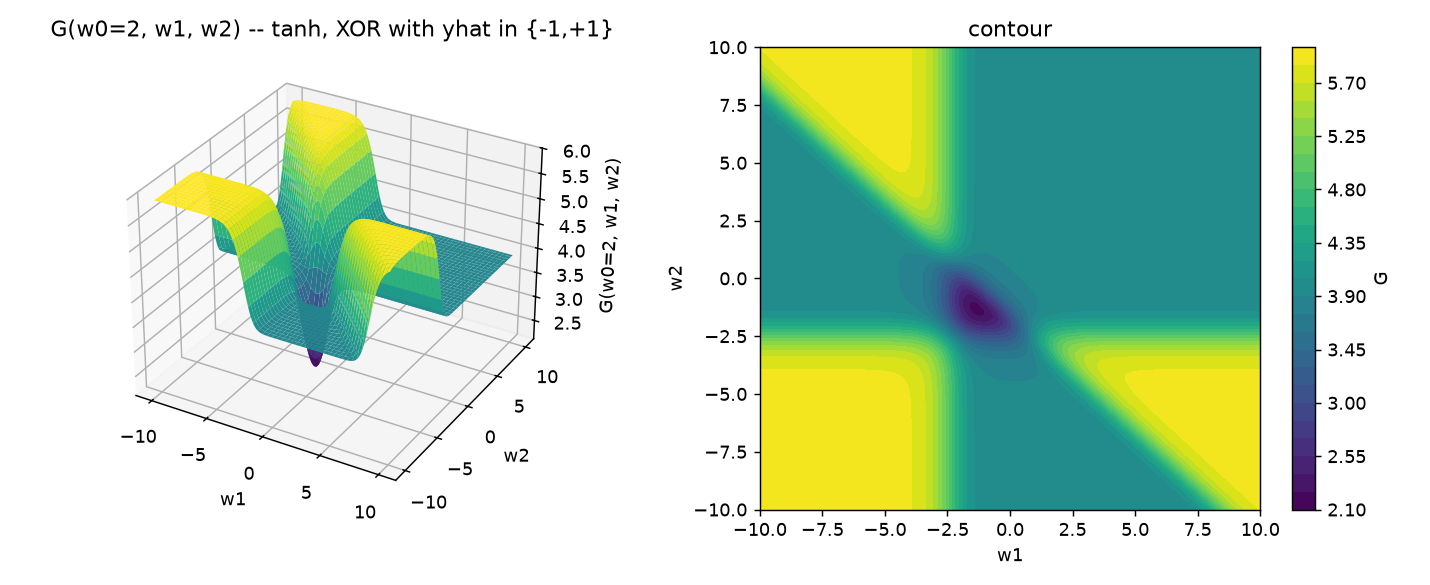
\includegraphics[width=\textwidth]{error_surface_main.png}
\end{center}

The surface has a single basin (minimum $G\approx2.19$ around $w_1\approx w_2\approx-1.36$) that never reaches
$0$: with $w_0$ fixed, $y$ is still just a linear function of $x_1,x_2$, so this is really
the same situation as Assignment 9 -- no choice of $w_1,w_2$ can realize XOR, the surface just shows how far
off the best possible linear fit remains.

\section*{Assignment 15}

AI use: I used Claude (Anthropic) to work through this part, as the sheet requires. I gave it the
assignment text directly and asked it to compare single-step and cumulative Backpropagation of Error. The
answer was usable as-is, so I didn't need to re-prompt or discard anything.

Single-step learning: One pattern $p$ is presented, its $\Delta w_{ij}$ computed,
and the weights are updated \emph{immediately}, before the next pattern is shown.

Cumulative learning: All $P$ training patterns are presented first, and their weight changes
${}^p\Delta w_{ij}$ are accumulated, $\Delta w_{ij}=\sum_{p=1}^P {}^p\Delta w_{ij}$, without touching the
weights; only after the full epoch is the sum applied once. This is exact gradient descent on the total error
$G=\sum_p {}^pE$.

\begin{itemize}
  \item Single-step: + many more updates per epoch, usually converges faster in wall-clock
  terms; the noise from updating on one pattern at a time can help escape shallow local minima; needs no extra
  memory to accumulate $\Delta w$; works for streaming data. \emph{--} the update direction is noisy and
  zig-zags (it follows one pattern's gradient, not $G$'s true gradient); the result depends on the order
  patterns are presented in.
  \item Cumulative: + follows the true gradient of $G$, so convergence is smooth and
  order-independent; easier to analyze with standard gradient-descent theory. \emph{--} requires a full pass
  over all patterns before a single update, so it's slower per update and needs more memory to accumulate
  $\Delta w$; with no stochastic noise it is more likely to get stuck exactly in a local minimum or saddle
  point; not applicable to online/streaming settings where the full pattern set isn't available upfront.
\end{itemize}

\end{document}
